\documentclass[border=10pt]{standalone}
\usepackage{karnaugh-map}
\usepackage{tikz}

\begin{document}
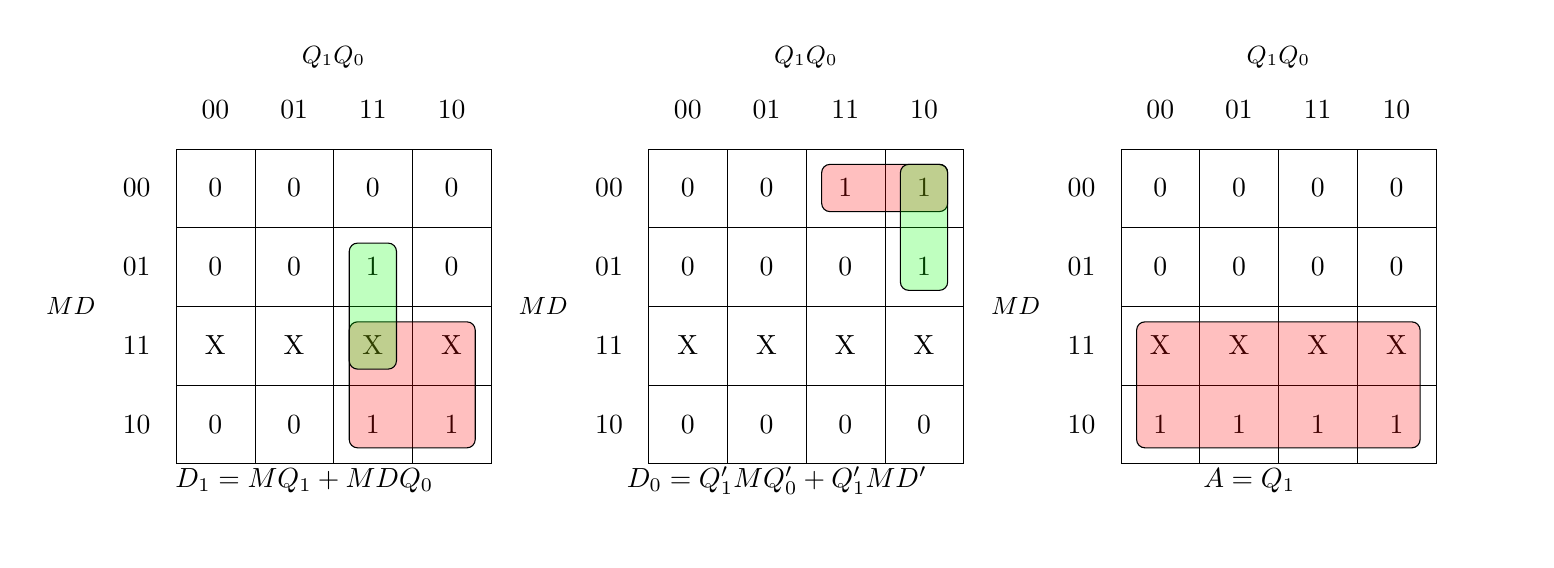
\begin{tikzpicture}
    % Variables: Rows Q1Q0, Cols MD
    % Q1Q0: 00, 01, 11, 10
    % MD:   00, 01, 11, 10
    % Indices: Standard Karnaugh 4 var (ABCD -> Q1 Q0 M D)
    
    % D1 (Next Q1)
    % Minterms: 7 (01 11), 10 (10 10), 11 (10 11)
    % Don't Care: 12, 13, 14, 15 (Row 11)
    \node at (0, 4) {
        \begin{karnaugh-map}[4][4][1][$Q_0$][$Q_1$][$D$][$M$]
            \minterms{7,10,11}
            \terms{12,13,14,15}{X}
            \autoterms[0]
            \implicant{15}{10} % Group 11,10,15,14 -> Q1 M
            \implicant{7}{15}  % Group 7,15 -> Q0 M D
        \end{karnaugh-map}
    };
    \node at (0, 1.5) {$D_1 = M Q_1 + M D Q_0$};

    % D0 (Next Q0)
    % Minterms: 2 (00 10), 3 (00 11), 6 (01 10)
    % Don't Care: 12, 13, 14, 15
    \node at (6, 4) {
        \begin{karnaugh-map}[4][4][1][$Q_0$][$Q_1$][$D$][$M$]
            \minterms{2,3,6}
            \terms{12,13,14,15}{X}
            \autoterms[0]
            % Groups
            \implicant{3}{2} % Q1' Q0' M
            \implicant{2}{6} % Q1' M D'
        \end{karnaugh-map}
    };
    \node at (6, 1.5) {$D_0 = Q_1' M Q_0' + Q_1' M D'$};
    
    % Output A
    % Minterms: 8,9,10,11 (Row 10)
    % Don't Care: 12,13,14,15 (Row 11)
    \node at (12, 4) {
        \begin{karnaugh-map}[4][4][1][$Q_0$][$Q_1$][$D$][$M$]
            \minterms{8,9,10,11}
            \terms{12,13,14,15}{X}
            \autoterms[0]
            \implicant{12}{10} % Rows 11 and 10 -> Q1
        \end{karnaugh-map}
    };
    \node at (12, 1.5) {$A = Q_1$};

\end{tikzpicture}
\end{document}
